\documentclass[11pt]{article}
\usepackage[a4paper, margin=20mm]{geometry}
\usepackage{setspace}
\usepackage{graphicx}
\usepackage{float}
\usepackage{eurosym}
\usepackage{amsmath}
\usepackage{longtable}
\usepackage{tikz}

\begin{document}
	\doublespacing
	
	\section{Demise Instrumentation}
	
	\paragraph{}The CubeSat is designed to test a different ablative material on each of its six exterior faces. To produce meaningful data for client use, each material sample will be equipped with its own dedicated sensor array. These arrays will measure temperature, pressure, and material recession through a combination of sensors and analogue-to-digital converters. All components are selected to be compatible with the I2C communication protocol, allowing for integration with the satellite’s onboard computer.
	
	\subsection{Component Choice}
	
	\subsubsection{Temperature}
	
	\paragraph{}Several methods exist for the evaluation of temperature.
	
	\begin{center}
		\begin{tabular}{|p{4cm}|p{5cm}|p{5cm}|}
			\hline
			\bf{Measurement Type} & \bf{Advantages} & \bf{Disadvantages} \\ \hline
			Infrared Camera & Provides a detailed view of temperature distribution over material surfaces & Expensive, difficult to position, and low frequency of measurement \\ \hline
			Heat Flux Sensor & Directly measures heat transfer, suitable for use on ablative material surface & Limited temperature range, and do not measure temperature directly \\ \hline
			Thermocouple & Can possess a wide temperature range, offer rapid response time, and is cost-effective & Only provides relative temperature difference (i.e. requires reference) \\ \hline
		\end{tabular}
	\end{center}
	
	\paragraph{}Given the above considerations, infrared cameras are non-ideal given their impracticality in a satellite context. Heat flux sensors, too, do not provide the data desired for this application. Thermocouples are commonly used in a space context, offer a high frequency of data acquisition and are relatively simplistic in their implementation.
	
	\paragraph{}Thermocouples operate based on the Seebeck effect, which measures the temperature difference between two points and generates an analogue voltage output in response. Among the various types available, Type K thermocouples are the most suitable for this context due to their wide temperature range and proven reliability in aerospace environments. A selection of viable sensors is summarised in the table below:
	
	\begin{center}
		\begin{tabular}{|p{4cm}|p{5cm}|p{5cm}|}
			\hline
			\bf{Product} & \bf{Temperature Range} & \bf{Notes} \\ \hline
			Collins Aerospace 0118MF &  -269°C to 400°C & \\ \hline
			Sensirion STS21 & -40°C to 125°C & Supply voltage 2.1 to 3.6V\\ \hline
			TE Connectivity MEAS 410 & -200°C to 1,250°C & Precision ±2.2°C\\ \hline
		\end{tabular}
	\end{center}
	
	\paragraph{}Of the options, the TE Connectivity MEAS 410 Thermocouple stands out as the most appropriate choice. Its wide temperature range of -200°C to 1,250°C can more effectively cope with the expected thermal extremes encountered in orbit. The device also offers acceptable precision and is well-suited for integration into satellite systems due to its straightforward electrical requirements and durability in harsh environments. As such, it represents a reliable solution for temperature monitoring with this application in mind.
	
	\paragraph{}This thermocouple requires an analogue-to-digital converter in order to be able to communicate its measurements. With standard type K thermocouple potential difference and temperature relations in mind~\cite{ref}, the operating voltage for the chosen thermocouple is likely to range between \(-5891~\mu {V}\) and \(50644~\mu V\), a fact that the ADC decision should rely on. Additionally, the thermocouple requires a cold junction (reference temperature) in order to measure the temperature of the test material. Many ADCs designed for use with thermocouples are made with CJC (Cold Junction Compensation). This feature creates a junction of known temperature for the thermocouple to use as a reference, simplifying the sensor array's design. The following are listed ADCs potentially usable with the MEAS 410 Thermocouple.
	
	\paragraph{}The selected thermocouple requires an analogue-to-digital converter (ADC) to transmit its measurements to the onboard system. Based on standard Type K thermocouple voltage–temperature characteristics [REF HERE], the expected output voltage range is approximately \(-5891~\mu {V}\) and \(50644~\mu V\). This range is a factor in selecting a suitable ADC. Additionally, accurate thermocouple measurements depend on a cold junction reference. Many ADCs designed for thermocouple use include integrated Cold Junction Compensation (CJC), which establishes a known reference temperature at the junction point. This feature greatly simplifies the overall sensor array design. A selection of ADCs compatible with the MEAS 410 thermocouple with large temperature ranges is listed below.
	
	\begin{center}
		\begin{tabular}{|p{4cm}|p{2.5cm}|p{2.5cm}|p{2cm}|p{2cm}|p{1cm}|}
			\hline
			\bf{Product} & \bf{Voltage Range} & \bf{Operating Temperature} & \bf{Resolution} & \bf{Interface} & \bf{CJC} \\ \hline
			Texas Instruments ADS1118IDGST& 0V to 4.096V & -40°C to 125°C & 12 bit & I2C & No\\ \hline
			ST Electronics RHFAD128 & -0.3 V to 4.8 V & -55°C to 125 °C & 12 bit & SPI & No \\ \hline
			Maxim MAX31856 & -0.3V to +4.0V & -55°C to 125°C & 19 bit & SPI & Yes\\ \hline
			Microchip MCP3421& -0.3V to 0.3V & -55°C to 125°C & 18 bit & I2C & No\\ \hline
			Texas Instruments ADS1115 & -0.3V to 0.3V & -40°C to 125°C & 16 bit & I2C & No \\ \hline
		\end{tabular}
	\end{center}
	
	\paragraph{} \paragraph{}None of the listed ADCs offer a perfect match for the application. The MAX31856 stands out with its appropriate voltage range and integrated Cold Junction Compensation, making it well-suited for thermocouple use. However, it communicates via the SPI protocol, which is not available directly on the CubeSat's onboard computer. In contrast, the MCP3421 supports the I2C interface, aligning well with the CubeSat’s existing communication protocol, and offers a compatible voltage range. Unfortunately, it lacks CJC.
	
	\paragraph{}Two potential solutions emerge to address the limitations of the ADC options. The first involves pairing the MAX31856 with an SPI-to-I2C bridge, such as the SC18IS602B. While this approach enables communication with the CubeSat's onboard computer, it introduces trade-offs. These include a reduced operational temperature range and potential constraints on data throughput. The second solution involves externalising Cold Junction Compensation by incorporating a dedicated temperature sensor to monitor the reference junction. Texas Instruments outlines such an approach [REF HERE], which enables accurate compensation through post-processing of the thermocouple signal.
	
	\paragraph{}The TMP36 is selected for this purpose. With an operating temperature range of -40°C to 125°C and a history in thermocouple applications, it is a reliable choice for monitoring the cold junction temperature. By integrating the TMP36 alongside a compatible ADC, Cold Junction Compensation can be implemented without relying on native ADC support.
	
	\subsubsection{Pressure}
	
	\paragraph{}Pressure sensors used in aerospace applications can vary significantly in size. However, the constraints of CubeSat engineering demand care to volume and mass minimisation. With these limitations in mind, the following sensor options have been selected for their compact size and practical suitability for integration within a CubeSat platform:
	
	\begin{center}
		\begin{tabular}{|p{4cm}|p{3cm}|p{3cm}|p{3cm}|}
			\hline
			\bf{Product} & \bf{Pressure Range} & \bf{Temperature Range} & \bf{Interface} \\ \hline
			Honeywell MPR Series & 60 mbar to 2.5 bar & 0°C to 50°C & I2C/SPI\\ \hline
			Honeywell MIP Series &  1 bar to 60 bar & -40°C to 125°C & I2C/SPI\\ \hline
			Sensata PTE7300 Series & & & \\ \hline
			& & & \\ \hline
		\end{tabular}
	\end{center}
	
	\paragraph{}MIPAG1XX002BAAAX
	
	
	\subsubsection{Recession}
	
	\paragraph{}Recession sensors are critical for measuring the ablation that occurs when the CubeSat surface is exposed to extreme conditions during reentry. These sensors are designed to quantify the rate at which a material is eroded over time, providing valuable data on its durability and performance under thermal stress. In the context of the CubeSat mission, recession sensors will be integrated into each material and will comprise part of its sensor array. By tracking the changes in the material’s thickness, the recession sensors will allow for a comprehensive understanding of the ablative properties of test materials.
	
	\paragraph{}Two main strategies exist to measure material recession. The first approach involves capacitive-based sensors, such as NASA’s Ablation Recession and Damage (ARAD) sensor or High Efficiency Ablation Thermography (HEAT) sensor[REF HERE]. These sensors are embedded perpendicular to the direction of ablation, with layered capacitive elements typically a dielectric material sandwiched between conductive plates. As the ablative material erodes, so too do the layers of the capacitor. This physical degradation results in a measurable reduction in capacitance, which can be correlated to the depth of material that has receded. This method allows for real-time monitoring of remaining ablative material, offering a direct and quantifiable insight into material performance under high thermal loads.
	
	\begin{figure}[H]
		\centering
		\includegraphics[width=0.5\textwidth]{ARAD.png}
		\caption{ARAD sensor electrical scheme [REF HERE]}
	\end{figure}
	
	
	\paragraph{}The other strategy is employed by ESA's ReWiG sensor. It includes a mesh of nickel wiring embedded into the ablative surface, positioned perpendicular to it. As the ablative material erodes during reentry, the mesh is similarly removed at an equal rate. This process allows the measurement of the sensor’s resistance, which in turn can be used to calculate the remaining thickness of the ablative material.
	\paragraph{}A key component of this system is the (also nickel) temperature compensation foil, which helps to account for temperature-induced changes in the resistance of the mesh. As the temperature fluctuates during reentry, both the mesh and the foil experience changes in their resistance. By comparing the resistance of the foil to that of the mesh, the sensor can isolate and correct for any temperature-related effects on the nickel mesh’s resistance. This ensures that the readings more accurately represent the erosion rate, accounting for thermal error to the resistance of the mesh.
	
	\begin{figure}[H]
		\centering
		\includegraphics[width=\textwidth]{ReWiG.png}
		\caption{ReWiG Sensor as seen in ESA report [REF HERE]}
	\end{figure}
	
	\paragraph{}A Howland current pump [REF HERE] is used to create a constant current source. EXPLANATION AND DESIGN GOES HERE
	
	\paragraph{}Once a constant current has been formed for each the mesh and foil of the recession sensor, an ADC is used to measure the voltage.
	
	\subsection{Data Rate}
	
	\begin{center}
		\begin{tabular}{|p{3.5cm}|p{3.5cm}|p{4cm}|p{3.5cm}|}
			\hline
			\bf{Sensor System} & \bf{Data rate} & \bf{Number of Sensors} & \bf{Total Data Rate}\\ \hline
			Temperature &   & &\\ \hline
			Pressure &  &  & \\ \hline
			Recession &  &  & \\ \hline
			\bf{Total} &  &  & \\ \hline
		\end{tabular}
	\end{center}
	
	
	\section{Interfacing and Communications}
	
	\paragraph{} A critical aspect of the mission's success is the CubeSat's ability to reliably transfer data from the sensor arrays to clients on the ground. To achieve this, the sensors are carefully selected to ensure integration with the onboard computer (OBC), while a reliable communications array is featured in the CubeSat design. The redundancy built into this data transmission process is crucial. Without the successful acquisition and transfer of this data to the ground, the mission would fail to yield results, eliminating the purpose of its investment.
	
	\subsection{Data System Architecture}
	
	\paragraph{} The CubeSat generates data through measurements taken by the sensor arrays, which include the thermocouple, pressure sensor, and recession sensor, as outlined in the instrumentation section. This sensor data is then relayed to the onboard computer (OBC), where it is processed, organised into data packets, and modulated for transmission through the communications array.
	
	\begin{figure}[H]
		\centering
		\includegraphics[width=\textwidth]{SystemOverview.png}
		\caption{System architecture overview illustrating data flow [GET UPDATED PHOTO]}
	\end{figure}
	
	\subsection{OBC and Data Processing}
	
	\paragraph{}One of the onboard computer's main  purposes within the context of this mission is to collect, collate and dispatch data. The selected OBC is the Ecuadorian Space Agency's ICEPS Spacecraft System Core, which offers a selection of desirable features, simplifying the CubeSat's design and ensuring a smooth flow of data.
	
	\begin{figure}[H]
		\centering
		\includegraphics[width=0.8\textwidth]{OBC.jpg}
		\caption{ICEPS Spacecraft System Core}
	\end{figure}
	
	\subsubsection{I2C Network}
	
	\paragraph{}The listed OBC features an Inter-Integrated Circuit (I2C) slave network, a serial communication protocol well-suited for compact embedded systems like in the CubeSat. I2C operates on a simple two-wire interface: a Serial Data Line (SDA) and a Serial Clock Line (SCL). This allows multiple slave devices (in this case, the analogue-to-digital converters corresponding to each sensor) to communicate with a single master, the OBC. Each slave device is assigned a unique address, enabling the OBC to selectively query and receive data from individual components without the need for extensive wiring. This significantly reduces system complexity and volume (important considerations in a CubeSat) while ensuring synchronised data acquisition across the sensor arrays. This topology and the ease of its integration make I2C an ideal choice for managing the CubeSat’s internal communication efficiently.
	
	\paragraph{}[PUT I2C DIAGRAM HERE]
	
	\paragraph{}Communication over I2C begins when the OBC, acting as the master, sends the address of the component whose response is needed,. If a device on the bus recognizes its address, it responds with an acknowledgement bit (ACK), allowing the OBC to verify that a device is present before proceeding. Once acknowledged, the OBC can initiate data transfer from the sensor, one byte (8 bits) at a time. After each byte, the OBC sends an ACK to confirm successful reception of the byte. The I2C protocol allows for sequential bytes to be sent in a single interaction, meaning that a device can return multiple bytes of data with consecutive messages and ACKs. This process ends when the master (OBC) ends the interaction and sends a new address. This approach makes I2C highly scalable, allowing the OBC to poll each sensor for its data as required.
	
	\paragraph{}
	
	\subsubsection{Software-Defined Radio}
	
	\paragraph{} Additionally, ICEPS can be provided with a Software-Defined Radio (SDR), which plays an important part in the CubeSat's communication system. The SDR is integrated within the OBC, enabling it to handle both the transmission and reception of data in a flexible, reconfigurable manner. Using software control, the SDR can be dynamically adjusted to work across different communication frequencies, modulation schemes, and protocols, making it adaptable for a variety of mission requirements. Once the OBC collects sensor data and processes it into packets, the SDR modulates the data for transmission over the L-Band.
	
	\paragraph{} ICEPS is designed for modularity, allowing adaptation to various mission requirements. The configuration options are as follows:
	
	\begin{center}
		\begin{tabular}{|p{12cm}|p{3cm}|}
			\hline
			\bf{Option} & \bf{Price (\euro)}\\ \hline
			FULL EPS ONLY (I2C INTERFACE) + 25W BATTERY & 20,500 \\ \hline
			FULL EPS (USB/I2C) + OBC/SDR RADIO/32GB SSD & 36,000 \\ \hline
			FULL EPS (USB/I2C) + OBC/SDR RADIO/256GB SSD + LASER COMMS & 45,000 \\ \hline
			FULL EPS (USB/I2C) + OBC/SDR RADIO/256GB SSD + LASER COMMS + D/R CONTROL & 50,000 \\ \hline
			FULL EPS (USB/I2C) + OBC/SDR RADIO/512GB SSD + LASER COMMS + D/R CONTROL + 25W BATTERY & 55,000 \\ \hline
			FULL EPS (USB/I2C) + OBC/SDR RADIO/512GB SSD + LASER COMMS + D/R CONTROL + 50W BATTERY & 58,000 \\ \hline
			FULL EPS (USB/I2C) + OBC/SDR RADIO/512GB SSD + LASER COMMS + D/R CONTROL + 100W BATTERY & 66,000 \\ \hline
		\end{tabular}
	\end{center}
	
	\paragraph{}The selected (second) configuration includes the SDR and EPS modules, with an external communications system implemented as detailed later in this report. This setup balances cost with system simplicity.
	
	\subsubsection{Communication Protocol}
	
	\paragraph{}[DISCUSS PACKET ORGANISATION FOR IRIDIUM SBD + PAYLOAD DESC]
	
	\begin{center}
		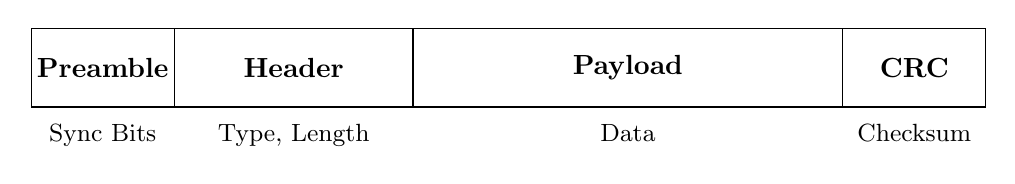
\begin{tikzpicture}
			\def\totalwidth{\linewidth}
			\def\preamblewidth{0.15*\totalwidth}
			\def\headerwidth{0.25*\totalwidth}
			\def\payloadwidth{0.45*\totalwidth}
			\def\crcwidth{0.15*\totalwidth}
			
			% Draw rectangles using relative widths
			\draw (0,0) rectangle ({\preamblewidth},1);
			\node at ({0.5*\preamblewidth},0.5) {\textbf{Preamble}};
			
			\draw ({\preamblewidth},0) rectangle ({\preamblewidth+\headerwidth},1);
			\node at ({\preamblewidth + 0.5*\headerwidth},0.5) {\textbf{Header}};
			
			\draw ({\preamblewidth+\headerwidth},0) rectangle ({\preamblewidth+\headerwidth+\payloadwidth},1);
			\node at ({\preamblewidth+\headerwidth + 0.5*\payloadwidth},0.5) {\textbf{Payload}};
			
			\draw ({\preamblewidth+\headerwidth+\payloadwidth},0) rectangle ({\preamblewidth+\headerwidth+\payloadwidth+\crcwidth},1);
			\node at ({\preamblewidth+\headerwidth+\payloadwidth + 0.5*\crcwidth},0.5) {\textbf{CRC}};
			
			% Optional labels below
			\node[anchor=north] at ({0.5*\preamblewidth}, -0.1) {\small Sync Bits};
			\node[anchor=north] at ({\preamblewidth + 0.5*\headerwidth}, -0.1) {\small Type, Length};
			\node[anchor=north] at ({\preamblewidth+\headerwidth + 0.5*\payloadwidth}, -0.1) {\small Data};
			\node[anchor=north] at ({\preamblewidth+\headerwidth+\payloadwidth + 0.5*\crcwidth}, -0.1) {\small Checksum};
		\end{tikzpicture}
		
		\vspace{0.5em}
		\textbf{Figure:} Example structure of a CubeSat communication packet.
	\end{center}
	
	\subsection{Telemetry Strategy}
	
	\paragraph{}A vital component of the data return process is the communications system. The chosen strategy involves uplinking mission data to the Iridium satellite constellation, which then relays the data to a ground-based station. This approach has been effective in previous missions, such as the QARMAN CubeSat developed by the Von Karman Institute, for the European Space Agency.
	
	\paragraph{} The Iridium constellation consists of 66 active low Earth orbit (LEO) satellites, providing global coverage for voice and data communications. Operating in the L-band, Iridium supports continuous, low-latency data transfer, suitable for this mission. Its global reach ensures reliable communication regardless of reentry location. Also, by transmitting signals upward and away from the CubeSat’s trajectory, the system can help overcome communication blackout caused by the plasma sheath formed during atmospheric reentry.
	
	\subsubsection{Plasma Sheath}
	
	\paragraph{} During atmospheric reentry, the CubeSat travels at hypersonic speeds, heating surrounding air to very high temperatures. This ionises the gases around the satellite, forming a plasma sheath: a layer of charged particles. This sheath can interfere with or completely block radio frequency signals, particularly in the UHF ranges, a circumstance known as a communication blackout. Given the mission centres around the collection of data during reentry, and that the CubeSat will not survive the process, communication despite the blackout becomes necessary. 
	
	\begin{figure}[H]
		\centering
		\includegraphics[width=0.5\textwidth]{TransVel.png}
		\caption{Transmission Coefficient through plasma sheath with velocity (Mao et al. 2022)}
	\end{figure}
	
	\paragraph{}According to the study by Mao et al. (2022) [REF HERE], transmission through the plasma sheath becomes more difficult with higher spacecraft velocity or frequency of communications. The signals get absorbed and reflected to higher degrees in these conditions.
	
	\paragraph{}[TALK ABOUT L-BAND COMMS, EXPLAIN WHERE ELECTRON DENSITY/COLLISION FREQUENCY CAME FROM]
	
	\paragraph{}One-dimensional electromagnetic wave propagation can be described mathematically as
	
	\[
	\mathbf{E}(x) = \mathbf{E}_0 e^{-(\alpha + j\beta)x},
	\]
	
	
	
	where \( \mathbf{E}(x) \) is the electric field vector at distance \( x \) into the plasma, \( \mathbf{E}_0 \) is the initial field, \( \alpha \) is the attenuation coefficient (causing decrease in amplitude), and \( \beta \) is the phase coefficient (causing phase shift).
	
	
	\paragraph{}The attenuation of an electromagnetic wave as it propagates through plasma can be determined [REF HERE] by considering the wave's frequency ($\omega$), the electron density ($n_e$), the collision frequency ($\nu$), and some physical constants.

	\[\omega_p = \sqrt{\frac{n_e q_e^2}{\epsilon_0 m_e}}\]	
	
	\[\alpha_p = k_0 \sqrt{\epsilon_r - |\epsilon_i|}\]
	
	\[\beta_p = k_0 \sqrt{\epsilon_r + |\epsilon_i|}\]
	
	\[\epsilon_r = 1 - \frac{\omega_p^2}{\omega^2 + \nu^2}\]
	
	\[\epsilon_i = \frac{\omega_p^2 \nu}{\omega (\omega^2 + \nu^2)}\]
	
	\subsubsection{Beamforming}
	
	\paragraph{} To mitigate the attenuation of radio signals typically occurring  during reentry, a high-gain communication system can be considered to maintain signal strength whilst keeping within reasonable power requirements. However, high-gain antennae are impractical for this mission due to their size, not appropriate to the volume requirements for the CubeSat. Additionally, their narrow beamwidth makes them unsuitable due to the satellite's tumbling. This can result in signal transmission being directed into the high-density plasma toward the CubeSat's direction of travel, rather than toward the wake region where communication is more feasible.
	
	\paragraph{}[INCLUDE BEAMFORMING FIGURE HERE]
	
	\paragraph{} One method of obtaining the high gain required for reliable data transmission while staying within the CubeSat’s size and power constraints is to use beamforming. Beamforming involves using an array of smaller antennae whose relative phases can be controlled to constructively interfere in a desired direction. This effectively steers the beam without the need for mechanical movement, allowing the system to achieve highly directional beams similar to those of a large high-gain antenna, but with significantly reduced physical size. In the context of a tumbling CubeSat, beamforming can also enable a dynamic transmission pattern, improving the likelihood of successful data delivery even despite the changing attitude of the satellite.
	
	\begin{figure}[H]
		\centering
		\includegraphics[width=0.5\textwidth]{beamform.png}
		\caption{Diagram illustrating change in distance travelled between signals from different beamforming elements }
	\end{figure}
	
	\paragraph{}Assume the case of a linear array of antennae. In the above diagram, the electromagnetic wave formed from the element on the left (of distance \(d\) from the right element) travels another \(d \sin(\beta)\). Therefore, in an array of \(M\) elements, signals arriving from a direction \(\beta\) cause different time delays based on the angle of arrival. These delays are determined by:
	
	
	
	
	\[
	\tau = \frac{d \sin(\beta)}{c}
	\]
	
	
	where \(d\) is the spacing between elements, and \(c\) is the speed of light.
	
	\paragraph{}To compensate for these delays (and allow parallel signals to be congruent), a steering vector \( \mathbf{a}(\beta) \) is applied.
	
	
	\[
	\mathbf{a}(\beta) = 
	\begin{bmatrix}
		1 & e^{-j \frac{2 \pi d \sin(\beta)}{\lambda}} & \dots & e^{-j \frac{2 \pi (M-1) d \sin(\beta)}{\lambda}}
	\end{bmatrix}^T,
	\]
	
	
	where \(\lambda\) is the signal wavelength. Each term corresponds to each antenna's phase change, ensuring the difference in distance travelled is accounted for. This steering vector is used to generate weights with which to multiply the input signal, allowing every antenna to transmit its corresponding signal.
		
	\begin{figure}[H]
		\centering
		\includegraphics[width=\textwidth]{antenna.png}
		\caption{ HXDC16010 SA00 Iridium Short Burst Data Antenna visualisation}
	\end{figure}
	
	\paragraph{} The selected antenna is the HXDC16010 SA00 Iridium SBD model, designed for use with the Iridium satellite network. It operates within the required frequency band of 1616 to 1626 MHz and provides a peak gain of 2 dBic. Its compact size, measuring 41.5 millimeters in length and 14 millimeters in diameter, makes it suitable for arrangement into an array configuration, allowing multiple units to be mounted within the limited volume of the CubeSat. The antenna is also engineered for harsh environments and maintains its performance even when positioned near other antennas.
	
	\paragraph{} [EXPLAIN PHASE SHIFTING]
	
	\paragraph{} MATLAB's Phased Array System Toolbox was used to simulate and visualise the radiation pattern of a uniform rectangular antenna array, designed to operate within the Iridium frequency band. A custom antenna element was defined using a cardioid-like magnitude pattern to model the chosen antenna. The element spacing was set to half the wavelength to minimise grating lobes but still maintain constructive interference. The toolbox was used to visualise the array geometry and compute beamforming weights using a steering vector corresponding to azimuth and elevation angles from user input. The resulting directional gain pattern was plotted in 3D, and the peak gain was provided to the user via output.
	
	\begin{figure}[H]
		\centering
		\includegraphics[width=0.6\textwidth]{2patt.png}
		\caption{Radiation pattern with 2x2 arrangement (azimuth angle = elevation angle = 30 degrees)}
	\end{figure}
	
	\begin{figure}[H]
		\centering
		\includegraphics[width=0.6\textwidth]{3patt.png}
		\caption{Radiation pattern with 3x3 arrangement (azimuth angle = elevation angle = 30 degrees)}
	\end{figure}
	

	\paragraph{} The simulated radiation patterns for two antenna configurations are shown above. The first pattern corresponds to a 2x2 array, which achieves a peak gain of 13.52 dB, while the second pattern is for a 3x3 array, providing a peak gain of 20.56 dB. In both cases, the element spacing is set to 92 mm, which is half of the wavelength at the operating L-band frequency, as previously discussed. As a result, the 3x3 configuration requires a larger physical area but offers the advantage of a higher peak gain.
	
	\paragraph{}[EXPLAIN TRADE-OFF (2x2/3x3?)]
	
	\paragraph{}Beamforming provides the CubeSat a higher gain, but assumes knowledge of the direction of the plasma sheath's wake.The CubeSat uses its communications array periodically to read an incoming signal from the nearest iridium satellite. It does this by reading signals from [FINISH PARAGRAPH]
	
	\paragraph{}Once the direction of transmission is known, the communications array is once again used to transmit data. Until the next occurrence of the direction measuring process, the onboard computer's in-built IMU is used to make slight adjustments to the array's directionality, recalculating the phase shifts for each antenna at every time-step [HOW OFTEN UPDATE?]. This allows for a reliable system due to the relatively low tumbling frequency [HOW LOW?] and cardioid-based radiation pattern from the antennae, granting the CubeSat flexibility in the direction of transmission.
	
	
	\subsubsection{Link Budget}
	
	\paragraph{}[DESCRIBE LINK BUDGET AND PURPOSE, WRITE CALCULATION]
	
	\section{Electrical Systems and Power}
	\subsection{OBC and Power Control}
	
	\paragraph{}[DESCRIBE POWER RAILS ON OBC]
	
	\subsubsection{Orbital Shut-off Period}
	
	\paragraph{}One of the primary challenges in designing the power system for this CubeSat is managing energy consumption during the long-duration orbital phase, which is expected to last approximately 23 days [CHECK THIS NUMBER IS RIGHT]. During this period, the spacecraft is inactive until the start of atmospheric re-entry. Even if the onboard computer (OBC) alone were to remain powered throughout this duration, the energy demands would be extreme. It draws an average 4 watts of power, which would lead to an energy requirement exceeding 2,000 watt-hours over the shut-off period. Therefore, an alternative mechanism is required to reliably reactivate the satellite in time for reentry while ensuring it is not drained of its energy before the mission is complete.
	
	\paragraph{}One potential approach considered was the use of a barometric sensor to detect the increasing air pressure associated with re-entry. However, this was quickly ruled out due to the pressure of the upper atmosphere. According to NASA atmospheric models[REF HERE], air pressure becomes effectively negligible above 20 km in altitude. This would not trigger a meaningful warning according to the planned trajectory for reentry [REF TO TRAJECTORY SECTION]. This, then, was not a suitable approach.
	
	\paragraph{}Another approach involved using a GPS module to determine the spacecraft’s altitude or orbital decay. A variety of GPS receivers designed for space were considered, including the u-blox NEO-M8 series, ZED-F9P, Trimble Copernicus, and Venus838LPx modules. While many of these modules are capable of functioning within the required temperature range, GPS modules consume significantly more power than expected, and may not function reliably during re-entry due to signal blackout. GPS-triggered reactivation was also ruled out for these reasons.
	
	\paragraph{}A more viable solution is the use of a low-power Real-Time Clock (RTC) module that remains active throughout the orbital period. Several RTC components were evaluated
	
	[DECIDE ON DEVICE]
	
	
	
	\paragraph{}The selected RTC module operates with power consumption of the order of just a few microwatts, leading to a negligible energy requirement over the orbital shut-off period. This is a highly efficient solution for ensuring the CubeSat can reactivate prior to re-entry. The minimal energy requirement also grants room for redundancy. Several RTC components [ADD DETAILS ON HOW MANY] are place into a majority-voting arrangement, lessening the capacity for a single-point failure in reactivation.
	
	\paragraph{}Due to the process of reactivation being scheduled, however, it may not take into account uncertainty with the trajectory and its
	
	\paragraph{}
	
	\subsection{Power Budget}
	
	\paragraph{}After reactivation, following the orbital shut-off period, the CubeSat's systems are powered and operational. The components are activated, and the process of data acquisition and transmission begins. The power budget for this operational phase of the mission is described below.
	
	\begin{longtable}{|p{3cm}|p{2cm}|p{2cm}|p{2cm}|p{3cm}|}
		\hline
		\textbf{Subsystem} & \textbf{Average Power (W)} & \textbf{Peak Power (W)} & \textbf{Duty Cycle (\%)} & \textbf{Avg. Power Usage (W)} \\
		\hline
		\endfirsthead
		
		\hline
		\textbf{Subsystem} & \textbf{Average Power (W)} & \textbf{Peak Power (W)} & \textbf{Duty Cycle (\%)} & \textbf{Avg. Power Usage (W)} \\
		\hline
		\endhead
		
		\hline
		\endfoot
		
		OBC &  &  & \% &  \\
		Temperature Sensors &  &  & \% &  \\
		Pressure Sensors &  &  & \% &  \\
		Recession Sensors &  &  & \% &  \\
		Comms Array &  &  & \% &  \\
		Spectrometer &  &  & \% &  \\
		Thrusters &  &  & \% &  \\
		\hline
		\textbf{Total} &  &  & & \textbf{0} \\
		\hline
		
	\end{longtable}
	
	\paragraph{}This section of the mission is planned to last for 1 hour [NOTE: UPDATE WHEN EXACT LENGTH IS KNOWN]. The total energy requirement for this phase is calculated as the sum of the energy consumed during the operational period and the energy required to support the system reactivation process after the shut-off period:
	
	\[
	E_{\text{total}} = P_{\text{avg}} \times t_{\text{operation}} + E_{\text{reactivation}}
	\]
	
	\noindent
	Where:  
	\begin{itemize}
		\item $E_{\text{total}}$ is the total minimum energy capacity required (Wh),
		\item $P_{\text{avg}}$ is the average power consumption during operation (W),
		\item $t_{\text{operation}}$ is the duration of this phase (hrs),
		\item $E_{\text{reactivation}}$ is the energy required to restore system functionality after shut-off (Wh).
	\end{itemize}
	
	\paragraph{}Substituting values in to find the energy requirement:
	
	\[
	E_{\text{total}} = (X \, \text{W}) \times (X \, \text{hr}) + X \, \text{Wh} = X \, \text{Wh}
	\]
	
	\paragraph{}Therefore, the minimum energy capacity required is \textbf{X watt-hours}.
	
	\paragraph{}[INTRO BATTERY AND CONNECTION TO OBC]
	
	
	\subsection{Power Distribution and System Design}
	
	\paragraph{}[SCHEMATIC GOES HERE]
	
	
\end{document}
